\documentclass{article}

\usepackage{graphicx} 
\usepackage[a4paper, total={6in, 10in}]{geometry}
\usepackage{multirow}
\usepackage[nobiblatex]{xurl}
\usepackage{amsmath}
\usepackage{float}

\graphicspath{{imgs/}}

\title{AI for Finance - Project 4}
\author{Eugenio Ferrari - mat. 239924}
\date{Spring 2023}

\begin{document}

\maketitle

\section{Intro}\label{sec:intro}

For the project I used the following libraries: \emph{Statsmodels} \cite{statsmodels}, \emph{Scikit-learn} \cite{scikit}. 

\vspace{1.5em}\noindent 
The goal of the project was to analyze loan default data and create a predictive model to determine whether a loan applicant is likely to default or not.

In this report, I will outline the steps taken during the project. Firstly, in Section \ref{sec:data-preprocessing}, I will discuss the data preprocessing part. Next, I will present the results of the five different AI models and logistic regression in Sections \ref{sec:ai} and \ref{sec:reg} respectively. The obtained results will be commented in Section \ref{sec:comments}.

In the last part of the report, I will focus on identifying the most important variables for the various models in Section \ref{sec:importance}. Finally, I will conclude the report in Section \ref{sec:webapp} by showcasing the developed demo web application.  

\section{Data Preprocessing}\label{sec:data-preprocessing}
The data preprocessing part was the most important step for the project, it involved:
\begin{itemize}    
    \item Handle missing data
    \item Handle categorical data
    \item Handle multicollinearity
    \item Handle unbalanced data    
\end{itemize}

\subsection{Missing Data}\label{subsec:missing-data}
After loading the data, I checked for missing data. I found only two variable with missing data, the first one: \emph{"person\_emp\_length"} had 895 missing entries, accounting for approximately 2.7\% of the data, so I decided to drop these rows. 

The  second variable was \emph{"loan\_int\_rate"}, but as described later in the report, I removed this variable due to its high correlation of 0.93 with another variable.

\subsection{Categorical Data}\label{subsec:cat-data}
After addressing missing data, the next step in the data preprocessing phase was encoding the categorical variables to prepare them for the models. I applied different techniques based on the nature of the variables:
\begin{itemize}
    \item \emph{"cb\_person\_default\_on\_file"}: For this variable, a simple mapping was used. "Y" was mapped to 1, indicating an historical default, and "N" was mapped to 0, indicating no default.
    \item \emph{"loan\_grade"}: Here I used an Ordinal Encoder, to preserve the ordinal relationship between the categories.
    \item \emph{"person\_home\_ownership"} and \emph{"loan\_intent"}: These variables were encoded using a One Hot Encoder.
\end{itemize}
By applying these encoding, categorical variables were transformed into numerical representations that can be effectively utilized by the models.

\subsection{Multicollineiarty}\label{subsec:multicollineiarty}
To address multicollinearity, a correlation matrix was generated by plotting the relationships between the variables. The correlation matrix is presented below in Figure \ref{fig:corr}. Based on this matrix, two variables, \emph{"cb\_person\_cred\_hist\_length"} and \emph{"loan\_int\_rate"}, showed a high correlation value ($>0.8$) with other variables. As a result, I made the decision to remove these variables from the dataset.

Additionally, another variable, \emph{"person\_home\_ownership\_MORTGAGE"}, showed a high correlation with \emph{"person\_home\_ownership\_RENT"}. However, since these variables are both derived from the same original variable and represent the one-hot encoding of different categories, I decided not to remove either of them.  
 
\begin{figure}[h!]
    \centering
    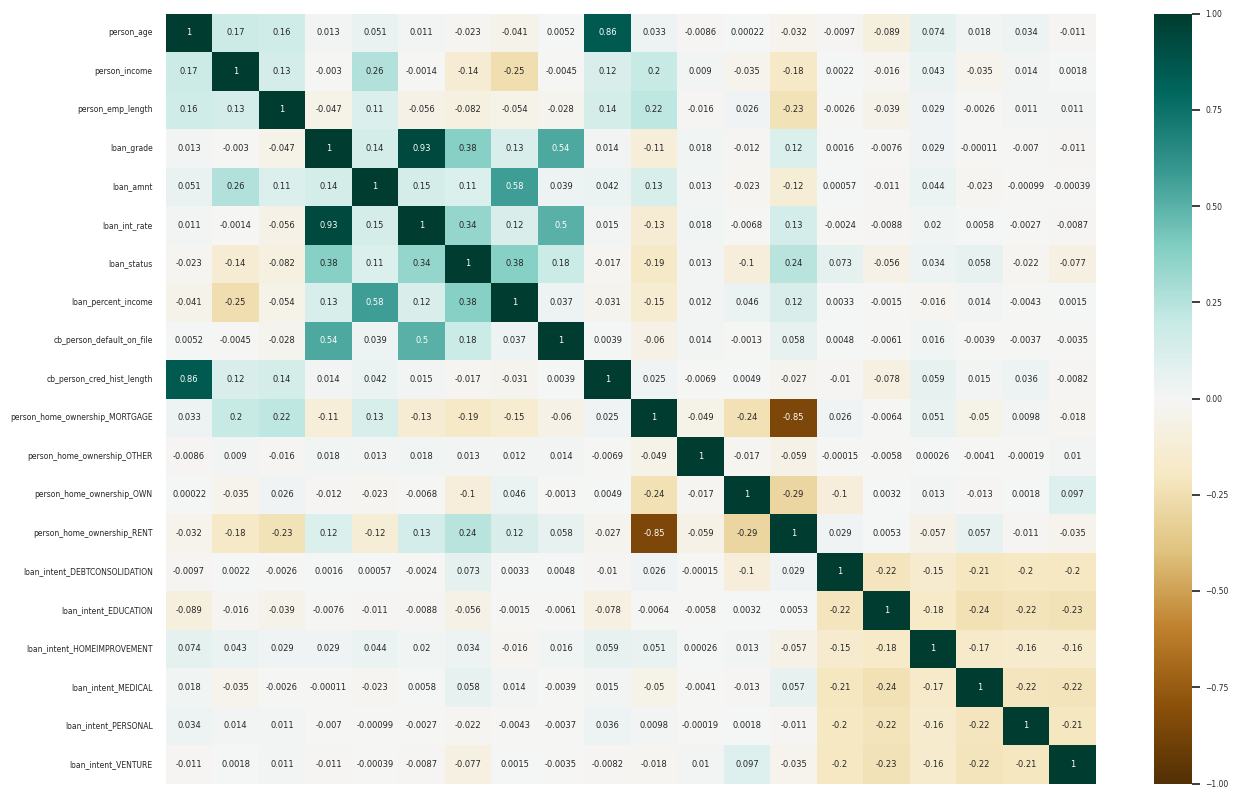
\includegraphics[width=\textwidth]{correlation.png}
    \caption{Correlation Matrix before removing multicollinearity}
    \label{fig:corr}
\end{figure}

\subsection{Unbalanced Data}\label{subsec:unbalanced-data}
Prior to splitting the data into training and validation sets and training the models, an important step was taken to address the issue of data imbalance. Figure \ref{fig:unbalance} illustrates the class distribution, indicating a significant majority of data points belonging to class 0 (no default).

To mitigate this problem and create a balanced dataset, I used the \emph{Synthetic Minority Over-sampling Technique (SMOTE)} \textbf{only on training data}. SMOTE generates synthetic samples for the minority class by interpolating between existing minority class samples. This process helped me balancing the class distribution and preventing bias towards the majority class during model training.

\begin{figure}[h!]
    \centering
    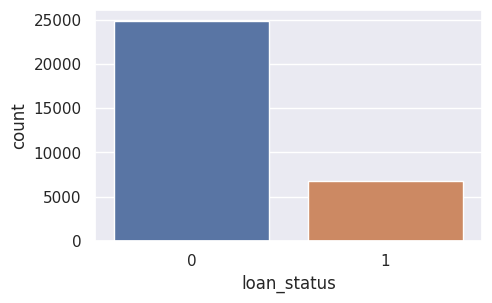
\includegraphics[width=0.4\textwidth]{unbalance.png}
    \caption{Unbalance in the dataset}
    \label{fig:unbalance}
\end{figure}

\newpage

\section{AI Models}\label{sec:ai}
I trained five different AI models and in this section, I will report for each model: the main hyperparameters, the accuracy and the confusion matrix. I will then comment these results in Section \ref{sec:comments}.

\subsection{Gaussian Naive Bayes}\label{subsec:gnb}
For this model I didn't set any hyperparameter.
\begin{itemize}
\item Accuracy: 0.55
\end{itemize}
\begin{figure}[h!]    
    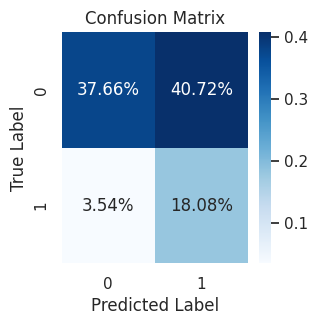
\includegraphics[width=0.38\textwidth]{gnb_cm.png}    
    \label{fig:gnb_cm}
\end{figure}

\subsection{Random Forest}\label{subsec:random-forest}
The Random Forest model was trained using the gini impurity criterion and consisted of 100 decision trees.
\begin{itemize}
\item Accuracy: 0.93
\end{itemize}
\begin{figure}[h!]    
    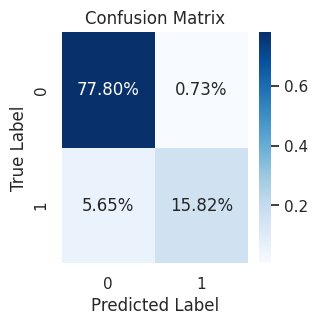
\includegraphics[width=0.38\textwidth]{rf_cm.png}    
    \label{fig:rf_cm}
\end{figure}

\subsection{AdaBoost Tree Ensamble}\label{subsec:adaboost}
The AdaBoost model used 50 decision trees with a learning rate of 1.0.
\begin{itemize}
\item Accuracy: 0.88
\end{itemize}
\begin{figure}[h!]    
    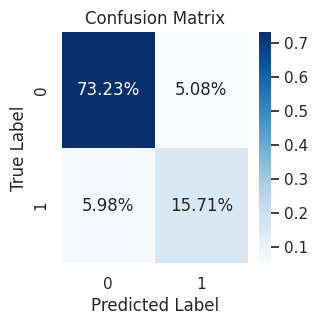
\includegraphics[width=0.38\textwidth]{adaboost_cm.png}    
    \label{fig:adaboost_cm}
\end{figure}

\newpage

\subsection{MLP}\label{subsec:mlp}
The MLP model utilized a hidden layer consisting of 50 neurons with the ReLU activation function and the Adam solver.
\begin{itemize}
\item Accuracy: 0.83
\end{itemize}
\begin{figure}[h!]    
    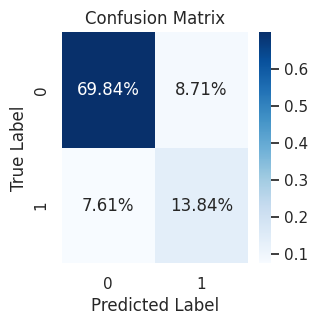
\includegraphics[width=0.38\textwidth]{mlp_cm.png}    
    \label{fig:mlp_cm}
\end{figure}

\subsection{SVM}\label{subsec:svm}
The SVM model employed an RBF kernel and a regularization parameter (C) value of 1.0.
\begin{itemize}
\item Accuracy: 0.75
\end{itemize}
\begin{figure}[h!]    
    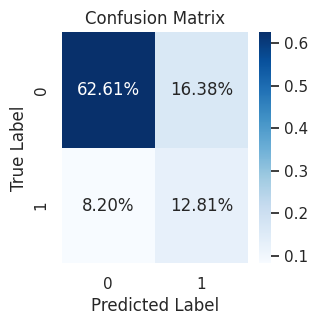
\includegraphics[width=0.38\textwidth]{svm_cm.png}    
    \label{fig:svm_cm}
\end{figure}

\newpage

\section{Logistic Regression}\label{sec:reg}
This are the results for the Logistic Regression model:
\begin{itemize}
\item Accuracy: 0.79
\end{itemize}
\begin{figure}[h!]    
    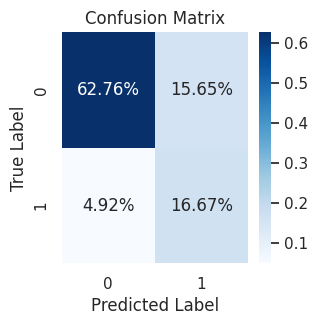
\includegraphics[width=0.38\textwidth]{reg_cm.png}    
    \label{fig:reg_cm}
\end{figure}

\section{Results Comments}\label{sec:comments}
\begin{itemize}
    \item The Random Forest model emerged as the best with an accuracy of 0.93.
    \item It is noteworthy that both the Random Forest and AdaBoost models, which are based on decision trees, demonstrated good performance. This can be attributed to the abundance of categorical features in the dataset. Decision tree-based models excel in handling categorical variables effectively, which likely contributed to their strong performance in this particular context.
    \item One issue encountered during the project was the problem of overfitting in all the models, leading to a tendency to predict the majority class due to the imbalance in the dataset. To address this issue, SMOTE was applied to the training data, as described in Section \ref{subsec:missing-data}. By generating synthetic samples for the minority class, SMOTE helped balance the dataset and alleviate the overfitting problem, enabling the models to learn from both classes more effectively.
    \item It is important to note that SMOTE was not applied to the test data to avoid artificially altering the original distribution of classes and overestimating the model's performance. As a result, the confusion matrix show a higher percentage in the top-left cell (True label = 0, Prediction = 0) due to the test set unbalance.
    \item In the next Section \ref{sec:importance}, I will talk about the variables importance.
\end{itemize}

\section{Variables Importance}\label{sec:importance}
To assess the contribution of variables to the prediction in the different models, various methods were employed based on the specific model characteristics.
For models based on decision trees, such as Random Forest and AdaBoost, the impurity-based feature importances learned during training were utilized. These feature importances provide insights into how much each variable contributes to reducing impurity within the decision trees, indicating their predictive significance.

For the other AI models, I used permutation importance. Permutation importance measures the decrease in model performance when a variable's values are randomly shuffled, providing an indication of its importance in the prediction process.

In the case of Logistic Regression, the significance of variables was evaluated using p-values and their statistical significance.

\vspace{1.5em}\noindent 
Below is a plot displaying the feature importances for the best-performing model, Random Forest. From the plot, we observe that the following features have the highest importance in predicting loan defaults:
\begin{enumerate}    
\item \emph{"loan\_grade"}
\item \emph{"loan\_percent\_income"}
\item \emph{"person\_income"}
\item \emph{"person\_home\_ownership"}
\item \emph{"cb\_person\_default\_on\_file"}
\item \emph{"loan\_amnt"}
\end{enumerate}

These features consistently demonstrate significant importance across most of the models. However, it's worth noting that the SVM model differs slightly, emphasizing only \emph{"person\_income"} and \emph{"loan\_amnt"} as the most influential features.

\begin{figure}[h!]
    \centering
    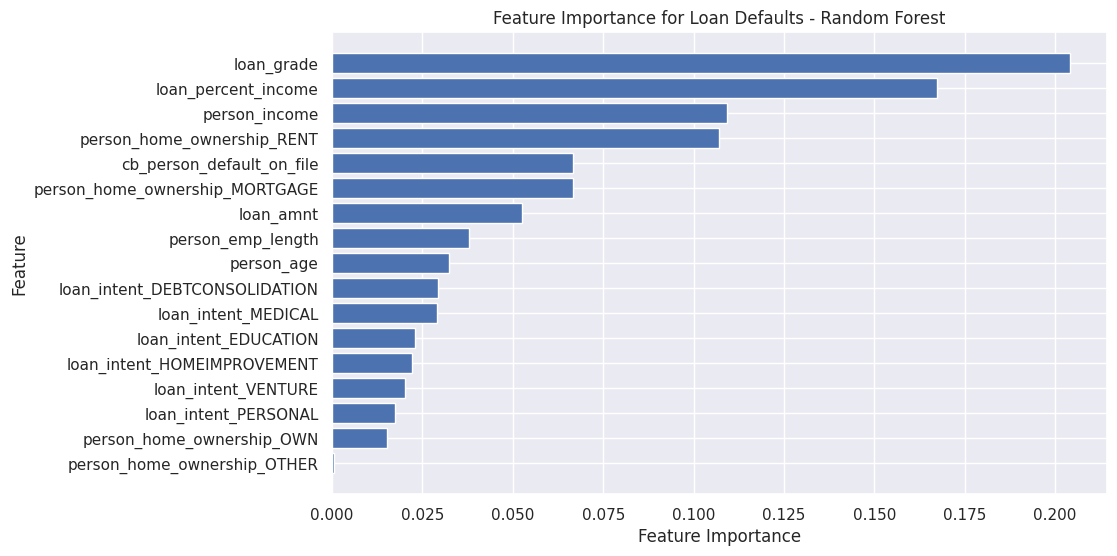
\includegraphics[width=\textwidth]{importance_rf.png}    
    \label{fig:importance_rf}
\end{figure}

\section{Webapp Demo}\label{sec:webapp}
The web application was developed using the \emph{Flask framework} \cite{flask}. The webapp is very simple: input textboxes where users can enter the data, and an output that displays the loan decision as "YES" or "NO". The deployed web application can be accessed at the following URL: 
\begin{itemize}
    \item \url{https://predict-loan-defaults.onrender.com/}.
\end{itemize}

To enable the deployment of the web application, the code was uploaded to a GitHub repository \url{https://github.com/eugenio24/predict-loan-defaults}. The deployment was facilitated using \emph{Render} \cite{render}, a cloud hosting service that allows for easy deployment of web applications.

Due to the utilization of the free hosting plan, the web application may experience a slow start initially (30/40 seconds). This delay can be attributed to the fact that the cloud instance on which the application is hosted shuts down during periods of inactivity to optimize resource usage. When a user accesses the web application after a period of inactivity, the cloud instance needs to be restarted, which can result in a slower start time. 

\subsection{Model used for the Demo}\label{subsec:model-demo}
For the web application, the best-performing model, Random Forest, was utilized, employing only the most important features. The selected features for the model are as follows:
\begin{itemize}
    \item \emph{"loan\_grade"}
    \item \emph{"loan\_percent\_income"}
    \item \emph{"person\_income"}
    \item \emph{"person\_home\_ownership"}
    \item \emph{"loan\_amnt"}
    \item \emph{"cb\_person\_default\_on\_file"}
\end{itemize}
Here is the accuracy and confusion matrix for this model:
\begin{itemize}
    \item Accuracy: 0.88
\end{itemize}
\begin{figure}[h!]
    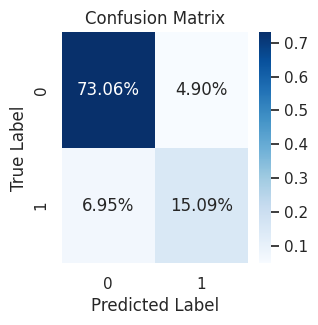
\includegraphics[width=0.4\textwidth]{cleaned_rf_cm.png}
    \label{fig:cleaned_rf_cm}
\end{figure}

\begin{thebibliography}{999}

\bibitem{statsmodels}
    Statsmodels, 
    \url{https://www.statsmodels.org/}
  
\bibitem{scikit}
    Scikit-learn,
    \url{https://scikit-learn.org/}

\bibitem{flask}
    Flask,
    \url{https://flask.palletsprojects.com/en/2.3.x/}

\bibitem{render}
    Render,
    \url{https://render.com/}
    
\end{thebibliography}
\end{document}